\documentclass[10pt]{article}
\usepackage{icmlko}

\icmlmeta{IP 파운데이션 월드모델}{333}{두 번째 줄}{같은 한 줄이 앨범 수집기에도 있었다 --- 그리고 검색은 그림자가 아니라 그냥 덜 긁은 것이었다}

\begin{document}

\twocolumn[
\icmlheader

\begin{abstract}
노트 332가 위키 수집기에서 풀 그림자를 한 줄 찾아 고쳤다. \textbf{남은
수집기를 다 뒤졌다.} 결과가 셋으로 갈린다.

\textbf{① 앨범 메타 --- 같은 한 줄이 또 있었다.}
\texttt{ingest/idol\_album\_meta.py} 의 \texttt{run()} 이
\texttt{pool = [r for r in recs if r["chodong\_basis\_resolved"] ==\
"hanteo"]} 다. 위키의 \texttt{idol\_items()} 와 \emph{같은 필터}가 다른
파일에 복사돼 있었다. 떼고 긁는 중이다(173건 중 124건까지).

\textbf{② 검색 --- 그림자가 아니었다.} \texttt{ingest/naver\_trend.py} 는
처음부터 \texttt{data/idol\_records} 를 직접 읽는다(필터 없음). 그런데
44건만 수집돼 있었다. \textbf{그냥 안 돌린 것이다.} 다 돌리니 169건이 되고
관측률이 한터 96\% · 추가 99\% 로 \texttt{poolshadow} 가 ``괜찮다''다.

\textbf{③ 다른 도메인 --- 다른 원인.} \texttt{ingest/trend\_all.py} 도
레코드를 읽는다. 도서의 검색 격차($+$80\%)는 필터가 아니라 데이터랩
시작일과 제목 조건에서 온다. \textbf{한 이름으로 부르면 안 되는 것이었다.}

\textbf{그리고 값이 또 나온다.} 같은 유보 25행에서

\begin{center}\footnotesize
\begin{tabular}{lrr}
\hline
 & 판 & 아이돌 \\
\hline
현행 \texttt{trendcalwikitag} & 0.4725 & 0.2385 \\
행만 넓힘 147행 & 0.4712 & 0.2831 \\
\quad $+$검색 & 0.4723 & 0.3585 \\
\quad $+$위키 & 0.4714 & 0.4469 \\
\quad \textbf{$+$둘 다} & \textbf{0.4763} & \textbf{0.5115} \\
\hline
\end{tabular}
\end{center}

\textbf{아이돌이 0.2385 에서 0.5115 로 두 배가 넘는다.} 짝지어(학습 재추출
열둘) 재면 위키 $+$0.2231(SD 0.0789 · \textbf{12/12}) · 검색
$+$0.0726(SD 0.1151 · 10/12) · 둘 다 $+$0.2632(SD 0.1072 ·
\textbf{12/12})이고 \textbf{판은 셋 다 $+$0.003 이하}(SD $\le$0.0030)로
안 움직인다. 아이돌은 판의 0.93\% 다.

\textbf{덤} --- 검색을 다 긁으니 \emph{현행 판}의 아이돌도 0.2108 $\to$
0.2385 로 올랐다. 축 파일 79행도 44/79 만 검색이 있었다.
\end{abstract}
]

\section{수집기를 다 뒤졌다}

\begin{center}\footnotesize
\begin{tabular}{lll}
\hline
수집기 & 후보를 어디서 & 판정 \\
\hline
\texttt{wiki\_views} & 축 파일 & \textbf{그림자}(332) \\
\texttt{idol\_album\_meta} & 레코드$+$\textbf{한터 필터} & \textbf{그림자} \\
\texttt{naver\_trend} & 레코드 & 게으름 \\
\texttt{trend\_all} & 레코드 & 다른 원인 \\
\hline
\end{tabular}
\end{center}

\textbf{같은 결과에 원인이 셋이다.} 노트 326이 관측률 표를 보고 ``풀의
그림자''라 이름 붙였을 때 넷을 한 이름으로 묶었는데, 실제로는 필터가 복사된
것 둘 · 안 돌린 것 하나 · 수집 조건이 다른 것 하나였다. \textbf{다음 수가
다르다} --- 필터는 떼고, 게으름은 돌리고, 조건은 못 고친다.

\begin{figure*}[t]
\centering
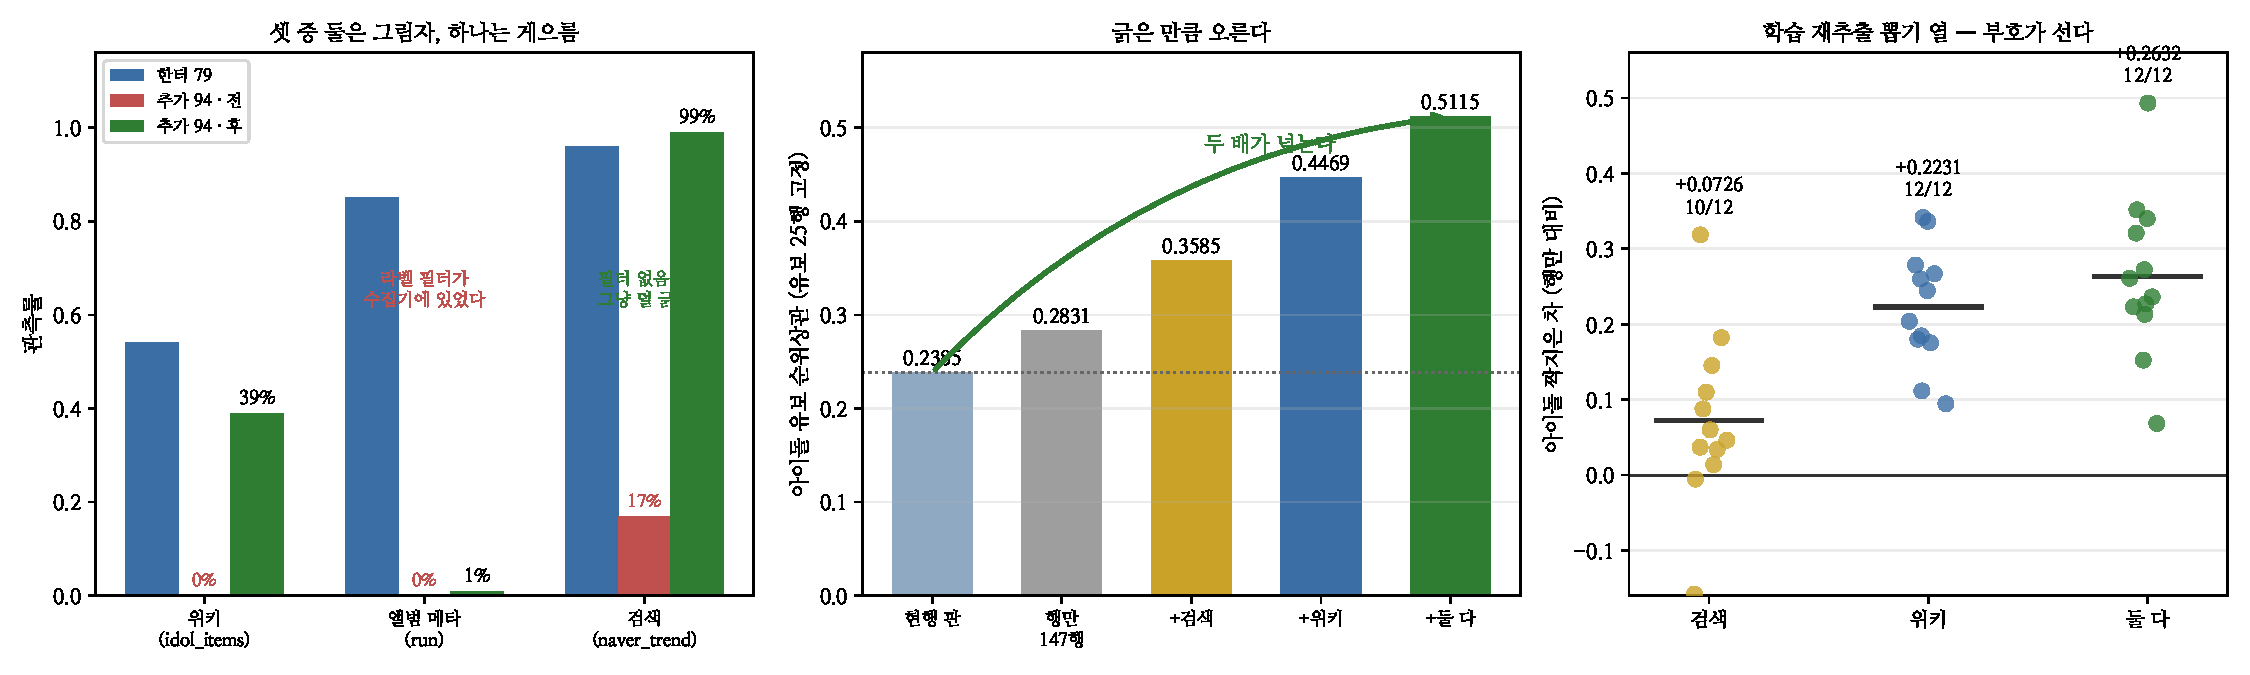
\includegraphics[width=\textwidth]{figs/lines.pdf}
\caption{왼쪽 --- 수집기 셋의 관측률. 가운데 --- 아이돌 사다리.
오른쪽 --- 짝지은 차.}
\end{figure*}

\section{검색은 그냥 안 돌린 것이었다}

\begin{center}\small
\begin{tabular}{lrr}
\hline
 & 전 & 후 \\
\hline
\texttt{idol\_trend.json} 키 & 44 & \textbf{169} \\
관측률 한터 79 & 35\% & \textbf{96\%} \\
관측률 추가 94 & 17\% & \textbf{99\%} \\
\texttt{poolshadow} 차 & $+$0.18 & \textbf{$-$0.03} \\
\hline
\end{tabular}
\end{center}

\textbf{추가 쪽이 오히려 높다.} 데뷔가 최근일수록 데이터랩 창에 들어가기
때문이다. \textbf{그림자가 아니라 게으름이었다} --- 그리고 게으름은
\emph{현행 판}도 갉아먹고 있었다. 축 파일 79행조차 44건만 있었다.

\section{사다리}

\begin{center}\footnotesize
\begin{tabular}{lrrr}
\hline
처치(행 넓힘 대비) & 평균 & SD & 양수 \\
\hline
$+$검색 & $+$0.0726 & 0.1151 & 10/12 \\
$+$위키 & $+$0.2231 & 0.0789 & \textbf{12/12} \\
\textbf{$+$둘 다} & \textbf{$+$0.2632} & 0.1072 & \textbf{12/12} \\
\hline
판(둘 다) & $+$0.0026 & 0.0017 & \\
\hline
\end{tabular}
\end{center}

\textbf{둘을 더한 것이 각각의 합보다 작다}($+$0.263 대 $+$0.296) --- 위키와
검색이 같은 것을 일부 잡는다. 노트 332에서 위키와 \emph{행}은 초가법이었는데
(합보다 $+$0.05 컸다) 위키와 \emph{검색}은 겹친다. \textbf{행은 자리를
늘리고 축은 서로 겹친다.}

\section{남은 것}
\begin{center}\footnotesize
\begin{tabular}{ll}
\hline
갈래 & 왜 \\
\hline
앨범 메타 긁기 끝내고 재라 & 마지막 그림자 · 지금 124/173 \\
\textbf{다른 도메인도 다 긁혔나} & 검색이 게을렀다면 딴 데도 \\
아이돌을 승격할까 & 판 안 움직이고 도메인 두 배 \\
값 대 표시자(검색) & 노트 332 규약 \\
\hline
\end{tabular}
\end{center}

\paragraph{규약} \textbf{같은 증상에 원인이 여럿이면 이름을 하나 더 붙이지
말고 원인마다 세라.} ``풀의 그림자''는 좋은 이름이었지만 넷을 묶는 바람에
\emph{하나는 그냥 안 돌린 것}이라는 제일 싼 사실을 여섯 노트 동안 못 봤다.
그리고 그 싼 것이 \textbf{현행 판까지 갉아먹고 있었다}(아이돌 0.2108 $\to$
0.2385). \textbf{설명이 그럴듯할수록 제일 시시한 가능성을 먼저 확인해야
한다} --- 여기서는 ``수집기를 끝까지 돌렸나''였다.

\end{document}
